\documentclass[11pt]{article}
\usepackage[utf8]{inputenc}
\usepackage{amsmath,amsthm,amsfonts,amssymb,amscd}
\usepackage{multirow,booktabs}
\usepackage[table]{xcolor}
\usepackage{fullpage}
\usepackage{lastpage}
\usepackage{enumitem}
\usepackage{fancyhdr}
\usepackage{mathrsfs}
\usepackage{wrapfig}
\usepackage{setspace}
\usepackage{calc}
\usepackage{multicol}
\usepackage{cancel}
\usepackage[retainorgcmds]{IEEEtrantools}
\usepackage[margin=3cm]{geometry}
\newlength{\tabcont}
\setlength{\parindent}{0.0in}
\setlength{\parskip}{0.05in}
\usepackage{empheq}
\usepackage{framed}
\usepackage[most]{tcolorbox}
\usepackage{xcolor}
\usepackage{blindtext}
\usepackage{hyperref}
\colorlet{shadecolor}{orange!15}
\parindent 0in
\parskip 12pt
\geometry{margin=1in, headsep=0.25in}
\theoremstyle{definition}
\newtheorem{defn}{Definition}
\newtheorem{reg}{Rule}
\newtheorem{exer}{Exercise}
\newtheorem{note}{Note}
\begin{document}
\setcounter{section}{0}
\title{Chapter 9 Review Notes}

\thispagestyle{empty}

\begin{center}
{\LARGE \bf Introduction to Variational Autoencoder}\\
{\large Group U8: Lake Yin, Zhiqi Wang}\\
Spring 2023\\
(\href{https://github.com/ZhiqiEliWang/csci4968-VAE-project}{https://github.com/ZhiqiEliWang/csci4968-VAE-projec})
\end{center}
\section{Motivation: From Autoencoder to Variational Autoencoder}
\subsection{Review on Autoencoder}
Autoencoder is a Deep Learning model that encode high dimensional information into latent space (encoder) to learn a lower dimension representation while ignoring the noise. 

In assignment 4, we've worked with a simple autoencoder model that encode the FashionMNIST dataset into 1 hidden layer and then reconstruct it to a output layer, which is the reconstructed image.

We could think about the latent space representation as features of an image, if we just use the generator of the autoencoder to generate a new image with the latent space representation, we could get a new image that is similar to the original image.

\section{Model of Variational Autoencoder}

\subsection{VAE structure From Autoencoder}
\begin{figure}[h]
    \begin{center}
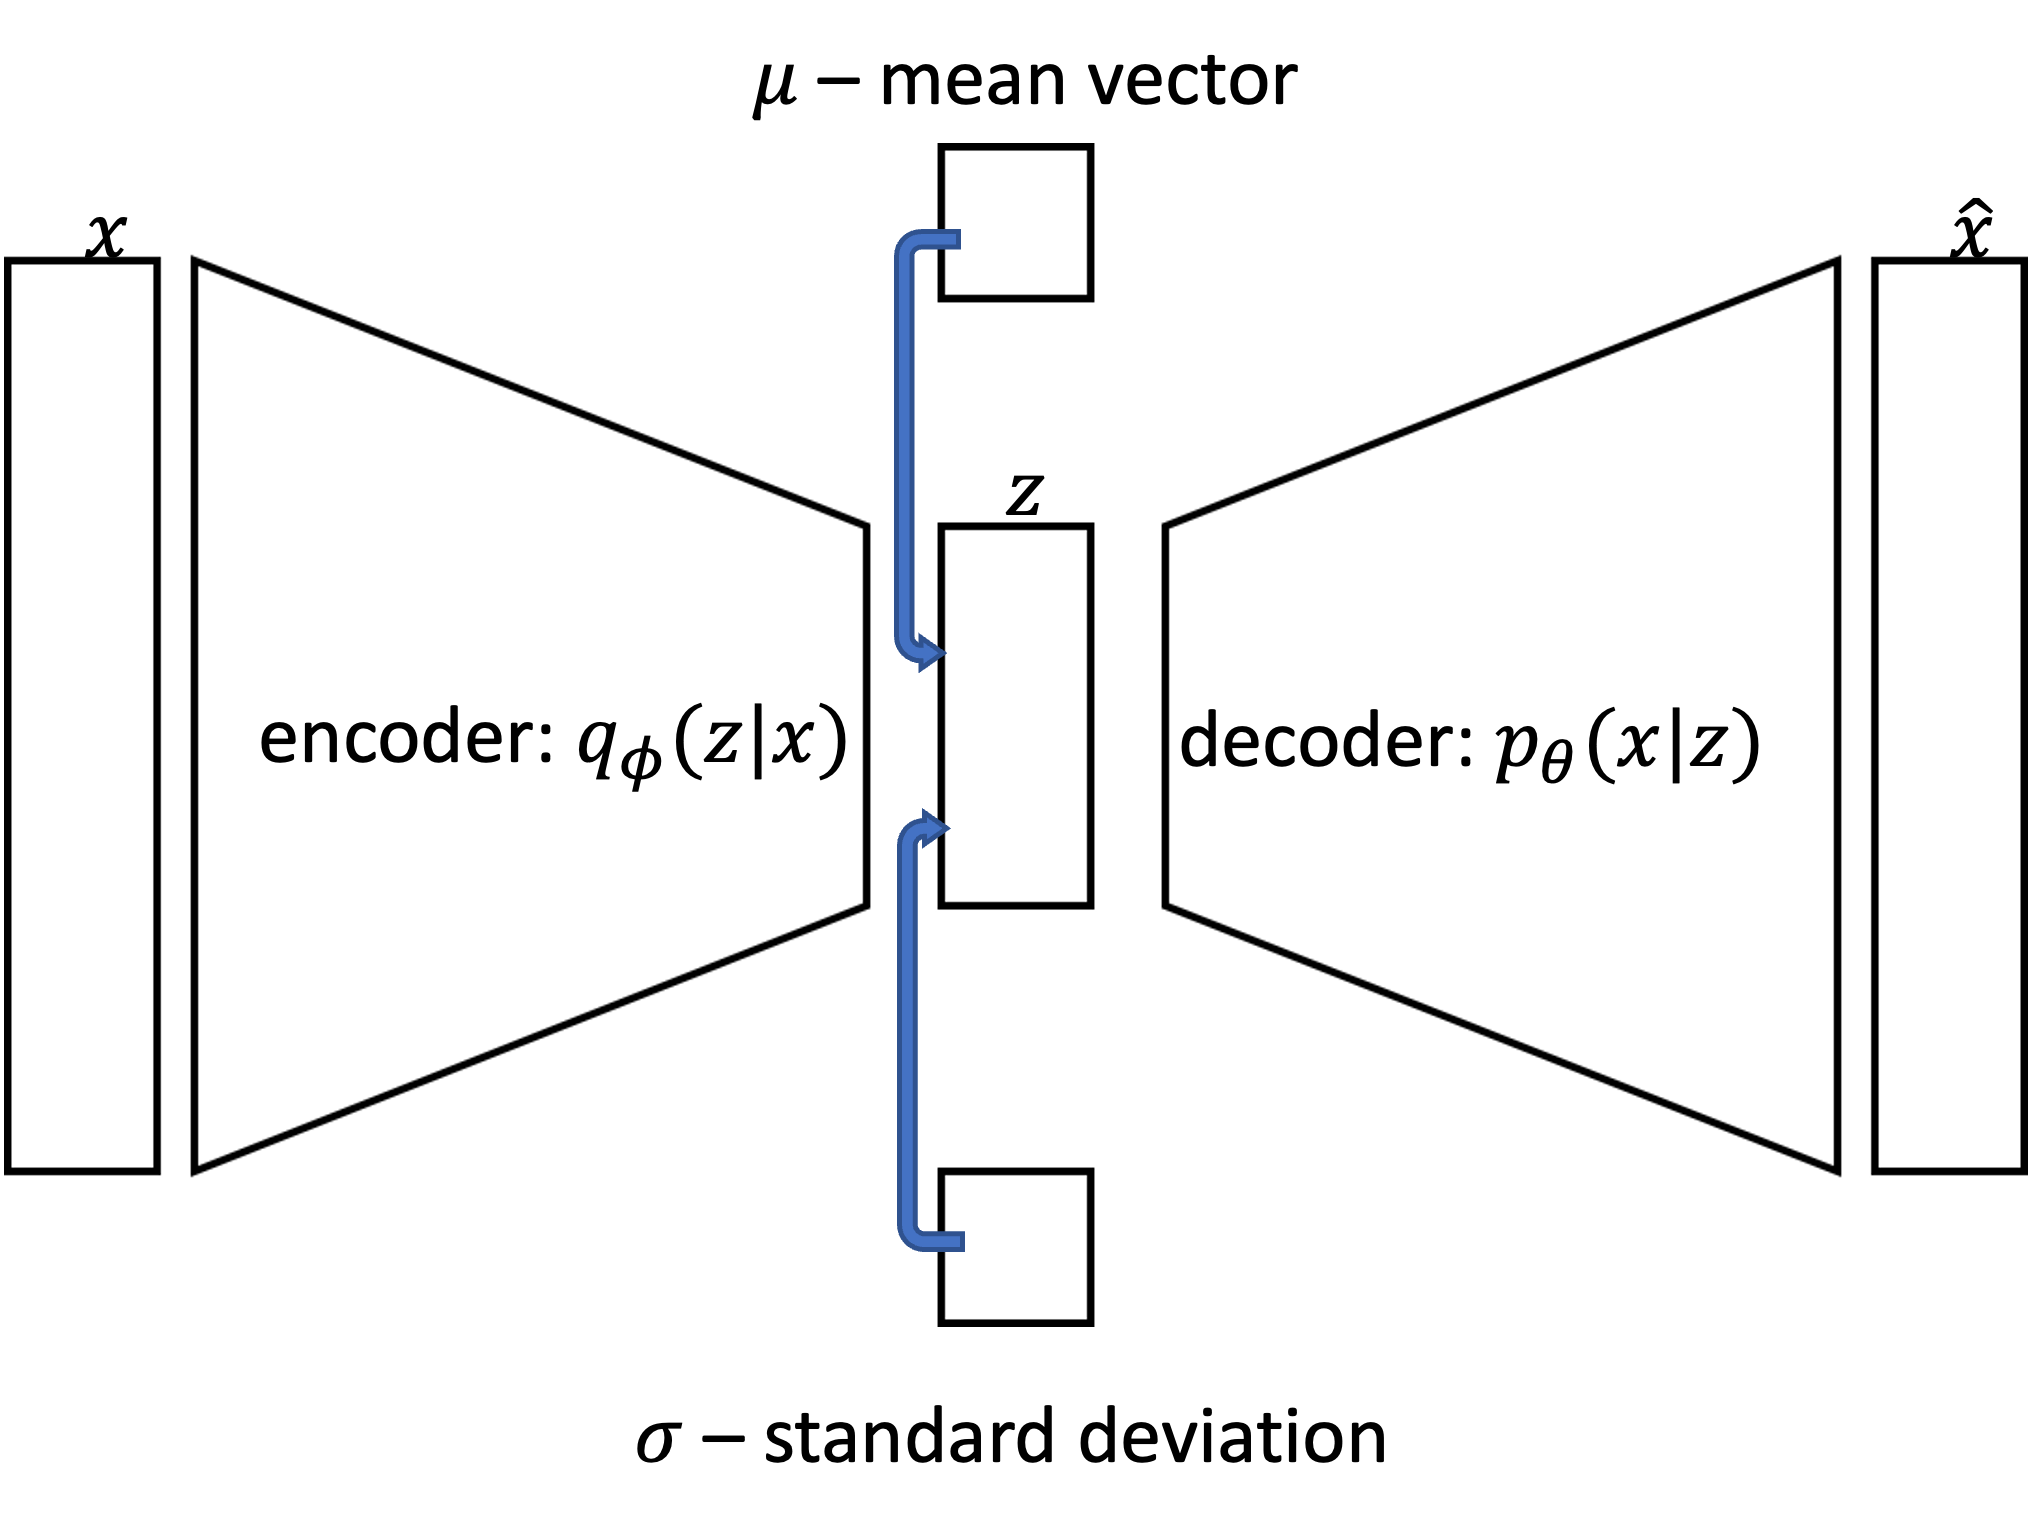
\includegraphics[scale=0.5]{vae-graph.png}
    \end{center}
\caption{VAE structure}
\end{figure}


For VAE to work, we need to make some assumption about the distribution of the latent space variable. We assume that the dataset $X$ is generated by some random process involving a unknown random variable $z$. This $z$ is generated from some prior distribution $q_{\theta^*}(z)$, and the data point $x \in X$ is generated from some conditional distribution $p_{\theta^*}(x|z)$. 

As the graph suggests above, we have a encoder that maps the data point $x$ to the latent space variable $z$, and a decoder that maps the latent space variable $z$ to the data point $\hat{x}$. What's different of this graph comparing to a classic autoencoder is that we have a prior distribution $p_{\theta}(z)$. A common choice for the prior distribution is a standard normal distribution. As the graph suggests, we have a mean vector and a standard deviation vector that maps the latent space variable $z$ to the mean and standard deviation of the distribution.

\subsection{Latent Variables}

Let's define latent variables as the variables that are not directly observed. In the case of VAE, the latent variables are the variables $z$ that are not directly observed. Since they are not observed in the input data, they are a part of our model. Therefore, we can model the observed data $x$'s distribution as a integral of the joint distribution of $x$ and $z$:

\begin{align}
    p_\theta(x) &= \int p_\theta(x, z) dz
\end{align}

$p_\theta(x)$ is called the marginal likelihood. If our goal is to find $\theta^*$ such that $p_{\theta^*}(x) \approx p*(x)$. We want to model the true distribution of $x$. 

\subsection{Intractabilities}

According to the definition of latent variables, we can model the observed data $x$'s distribution as a integral of the joint distribution of $x$ and $z$. However, this integral is intractable since we don't know the true distribution of $z$. 

Also, the posterior distribution 
\begin{align}
    p_\theta(z|x) &= \frac{p_\theta(x, z)}{p_\theta(x)}
\end{align}
is intractable since we know that $p_\theta(x)$ is intractable. To model the distribution of $x$, we could use VAE.


\subsection{VAE's objective function}

We introduce a parametric inference model $q_\phi(z|x)$, which corresponds to the encoder in the of autoencoder/VAE. We want to find $\phi^*$ such that $q_{\phi^*}(z|x) \approx p_\theta^*(z|x)$.

To find $\phi^*$, we want to minimize the KL divergence between $q_\phi(z|x)$ and $p_\theta^*(z|x)$:

\begin{align}
    \text{KL}(q_\phi(z|x)||p_\theta^*(z|x)) &= -\sum_{z} q_\phi(z|x) \log \frac{p_\theta^*(z|x)}{q_\phi(z|x)} \\
    p(z|x) = \frac{p(x|z) p(z)}{p(x)} &= \frac{p(x, z)}{p(x)}\\
    \text{KL}(q_\phi(z|x)||p_\theta^*(z|x)) &= -\sum_{z} q_\phi(z|x) \log \frac{p_\theta^*(x, z)}{p_\theta^*(x)q_\phi(z|x)} \\
    \text{KL}(q_\phi(z|x)||p_\theta^*(z|x)) &= -\sum_{z} q_\phi(z|x) \log \left[ \frac{p_\theta^*(x, z)}{q_\phi(z|x)}\cdot\frac{1}{p_\theta(x)}\right] \\
    \text{KL}(q_\phi(z|x)||p_\theta^*(z|x)) &= -\sum_{z} q_\phi(z|x) \log \frac{p_\theta^*(x, z)}{q_\phi(z|x)} + \sum_{z} q_\phi(z|x) \log p_\theta(x) \\
    \text{KL}(q_\phi(z|x)||p_\theta^*(z|x)) &= -\sum_{z} q_\phi(z|x) \log \frac{p_\theta^*(x, z)}{q_\phi(z|x)} + \log p_\theta(x)
\end{align}

The first term in RHS in equation (8) is the ELBO (Evidence Lower Bound) and we write it as $\mathcal{L}_{\phi, \theta}(x)$. Our goal is to minimize the KL divergence between $q_\phi(z|x)$ and $p_\theta^*(z|x)$, which is equivalent to maximizing the ELBO acoording to (8).

We can rearrange equation (8) to get:

\begin{align}
    \mathcal{L}_{\phi, \theta}(x) &= \log p_\theta(x|z) - D_\text{KL}(q_\phi(z|x)||p_{\theta^*}(z|x))
\end{align}


We could also simplify the ELBO from equation (8) as :
\begin{align}
    \mathcal{L}_{\phi, \theta}(x) &=\sum_{z} q_\phi(z|x) \log \frac{p_\theta^*(x, z)}{q_\phi(z|x)}\\
    &= \mathbb{E}_{q_\phi(z|x)}[\log p_\theta(x|z)] - \mathbb{E}_{q_\phi(z|x)}[\log q_\phi(z|x)]\\
    &= \mathbb{E}_{q_\phi(z|x)}[\log p_\theta(x|z) - \log q_\phi(z|x)]
\end{align}


\section{SGD and Reparameterization Trick}

\subsection{SGD}

The objective function of VAE is a non-convex function, so we need to use SGD to optimize the objective function. The objective function, when training with a batch of data, is:

\begin{align}
    \mathcal{L}_{\phi, \theta}(D) = \frac{1}{|D|}\sum_{x \in D} \mathcal{L}_{\phi, \theta}(x)
\end{align}

And the gradient of the objective function w.r.t. the generative model parameters $\theta$ is:
\begin{align}
    \nabla_\theta \mathcal{L}_{\phi, \theta}(x) &= \nabla_\theta\mathbb{E}_{q_\phi(z|x)}[\log p_\theta(x|z) - \log q_\phi(z|x)]\\
    &= \mathbb{E}_{q_\phi(z|x)}[\nabla_\theta\log p_\theta(x|z) - \nabla_\theta\log q_\phi(z|x)]\\
    &\approx \nabla_\theta(\log p_\theta(x|z) - \log q_\phi(z|x))\\
    &= \nabla_\theta\log p_\theta(x|z)
\end{align}

And the gradient of the objective function w.r.t. the variational parameters $\phi$ is harder to approach, since:
\begin{align}
    \nabla_\phi \mathcal{L}_{\phi, \theta}(x) &= \nabla_\phi\mathbb{E}_{q_\phi(z|x)}[\log p_\theta(x|z) - \log q_\phi(z|x)]\\
    &\neq \mathbb{E}_{q_\phi(z|x)}[\nabla_\phi\log p_\theta(x|z) - \nabla_\phi\log q_\phi(z|x)]
\end{align}

This is because $z$ is a stochastic variable in VAE that follows a prior distribution. So we can't directly calculate the gradient of the objective function w.r.t. $\phi$.

\subsection{Reparameterization Trick}

To solve the problem of the stochastic gradient, we can express the random variable $z$ as a deterministic function of the variational parameters $\phi$, the data point $x$, and a random variable $\epsilon$ that is sampled from a prior distribution $p(\epsilon)$:
\begin{align}
    z=g_\phi(x, \epsilon, \phi)
\end{align}
This is called the reparameterization trick, and the $\epsilon$ is usually sampled from a standard normal distribution $p(\epsilon) \sim \mathcal{N}(0, 1)$.

\subsection{Gradient of Expectation with Reparameterization Trick}

Given the change of variable $z=g_\phi(x, \epsilon, \phi)$, we can rewrite the gradient of the objective function w.r.t. the variational parameters $\phi$ as:

\begin{align}
    \mathbb{E}_{q_\phi(z|x)}[f(z)] = \mathbb{E}_{p(\epsilon)}[f(g(x, \epsilon, \phi))] = \mathbb{E}_{p(\epsilon)}[f(z)]
\end{align}

Then we could take gradient of equation (13) w.r.t. $\phi$:
\begin{align}
    \nabla_\phi \mathbb{E}_{q_\phi(z|x)}[f(z)] &= \nabla_\phi \mathbb{E}_{p(\epsilon)}[f(z)]\\
    &= \mathbb{E}_{p(\epsilon)}[\nabla_\phi f(z)]\\
    &\approx \nabla_\phi f(z)
\end{align}

\begin{figure}[h]
\includegraphics*[width=\textwidth]{reparam.png}
\caption{Reparameterization trick demonstration: on the left is the original form (without) reparameterization trick, and on the right is the reparameterization trick form. As it can be seen, the reparameterization trick enables us to take gradient of the expectation w.r.t. the variational parameters $\phi$, therefore we can backprogagate the gradient to the generative model parameters $\theta$.}
\end{figure}

\subsection{Gradient of Objective Function with Reparameterization Trick}

Now we can take gradient of the objective function w.r.t. the variational parameters $\phi$:
\begin{align}
    \mathcal{L}_{\theta, \phi}(x) &= \mathbb{E}_{q_\phi(z|x)}[\log p_\theta(x|z) - \log q_\phi(z|x)]\\
    &= \mathbb{E}_{p(\epsilon)}[\log p_\theta(x|z) - \log q_\phi(z|x)]
\end{align}

From equation (26), we can form our ELBO in with the reparameterized parameter $z$:

\begin{align}
    \epsilon &\sim p(\epsilon)\\
    z &= g_\phi(x, \epsilon, \phi)\\
    \mathcal{\tilde{L}}_{\theta, \phi}(x) &= \log p_\theta(x|z) - \log q_\phi(z|x)
\end{align}

$\mathcal{\tilde{L}}_{\theta, \phi}(x)$ is a Monte Carlo estimator of the objective ELBO of a single data point $x$ now we could use it for SGD.

\section{Further Reading}

This lecture note is based on the following papers:

\begin{itemize}
    \item \href{https://arxiv.org/abs/1312.6114}{Auto-Encoding Variational Bayes}
    \item \href{https://arxiv.org/abs/1906.02691}{An Introduction to Variational Autoencoders}
\end{itemize}

We started from autoencoder to variational autoencoder, then we defined the objective based on the encoder-decoder structure, and then we derived the reparameterization trick. The original paper of VAE is a bit hard to understand since it started with the motivation from probability, so I hope this lecture note can help you understand the VAE better.

\end{document}